\documentclass[border=12pt]{standalone}
\usepackage{tikz}
\usetikzlibrary{positioning,shapes,arrows.meta}

\begin{document}
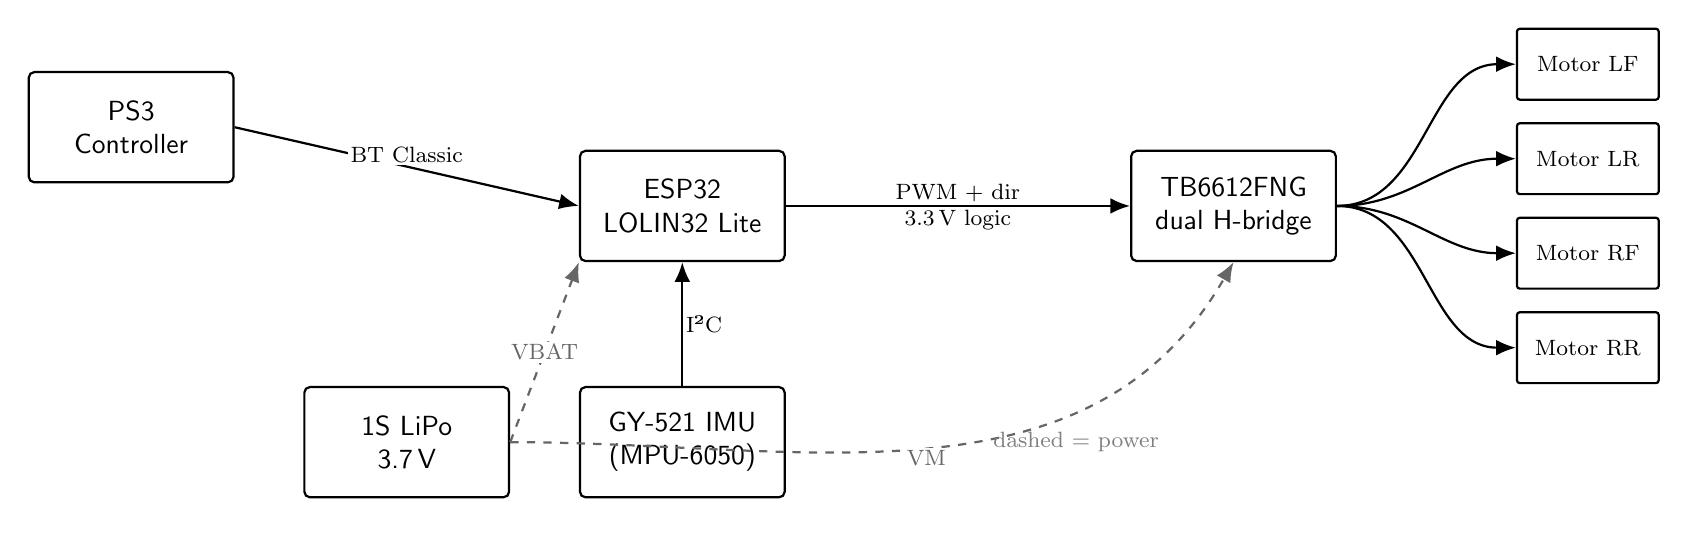
\begin{tikzpicture}[
  font=\sffamily,
  module/.style={
    draw, thick, rounded corners=2pt,
    minimum width=2.6cm, minimum height=1.4cm,
    align=center, fill=white,
  },
  small/.style={
    draw, thick, rounded corners=1pt,
    minimum width=1.8cm, minimum height=0.9cm,
    align=center, fill=white, font=\footnotesize,
  },
  bus/.style={-{Latex[length=2.5mm,width=2mm]}, thick},
  power/.style={-{Latex[length=2.5mm,width=2mm]}, thick, dashed, color=black!60},
  ann/.style={font=\footnotesize, fill=white, inner sep=1pt},
]

\node[module] (ps3) at (-7,1) {PS3\\Controller};
\node[module] (esp) at (0,0) {ESP32\\LOLIN32 Lite};
\node[module] (drv) at (7,0) {TB6612FNG\\dual H-bridge};
\node[module] (imu) at (0,-3) {GY-521 IMU\\(MPU-6050)};
\node[module] (bat) at (-3.5,-3) {1S LiPo\\3.7\,V};
\node[small] (mlf) at (11.5, 1.8) {Motor LF};
\node[small] (mlr) at (11.5, 0.6) {Motor LR};
\node[small] (mrf) at (11.5,-0.6) {Motor RF};
\node[small] (mrr) at (11.5,-1.8) {Motor RR};

\draw[bus] (ps3.east) -- node[ann,above]{BT Classic} (esp.west);
\draw[bus] (imu.north) -- node[ann,right]{I²C} (esp.south);
\draw[bus] (esp.east) -- node[ann,above]{PWM + dir} node[ann,below]{3.3\,V logic} (drv.west);
\draw[power] (bat.east) -- node[ann]{VBAT} (esp.south west);
\draw[power] (bat.east) to[out=0,in=240] node[ann,below]{VM} (drv.south);

\draw[bus] (drv.east) to[out=0,in=180] (mlf.west);
\draw[bus] (drv.east) to[out=0,in=180] (mlr.west);
\draw[bus] (drv.east) to[out=0,in=180] (mrf.west);
\draw[bus] (drv.east) to[out=0,in=180] (mrr.west);

\node[font=\footnotesize, color=black!50] at (5, -3) {dashed = power};

\end{tikzpicture}
\end{document}
